\chapter{Domino-Datenbank}

Die Informationen für dieses Kapitel wurden aus\cite{ebel} und \cite{knaepper} entnommen, sofern nicht anders angegeben.
%-------------------------------

\section{Allgemeine Beschreibung}
\label{sec:3dominoDB}

Eine Domino Datenbank auch als Notes Datenbank bezeichnet, enthält alle Daten und Informationen einer Anwendung. 
Die Datenstruktur, Funktionalität und die Oberfläche werden durch das Design einer Anwendung festgelegt. Eine Datenbankdatei
kann als eine Art Container gesehen werden. In diesem Container sind Gestaltungs-/Design-Elemente, sowie auch die Daten der Anwendung abgelegt\cite{ebel}.
Domino-Datenbanken sind die Grundbausteine einer Domino-Anwendung. Sie unterscheiden sich jedoch von klassischen Datenbanken.
Während klassische Datenbanken eine reine Ansammlung von Daten sind, können Domino-Datenbanken auch beliebig gestaltet werden. 
Eine Domino-Datenbank ist eine Ansammlung von miteinander in sachlicher Beziehung stehenden Dokumenten. Jedes Dokument wiederum besteht  
aus einem oder mehreren Feldern\cite{knaepper}. \newline
%
%Domino-Dokumente sind mit einer relationalen Datenbank vergleichbar, mit dem Unterschied, dass bei Domino die Programmierlogik, und die
%Gestaltungselemente in Form von Dokumenten verwaltet werden.\newline
Eine Domino-Datenbank ist \textbf{keine} Datenbank im herk\"ommlichen Sinn, sondern eine fertige Applikation, welche eine spezielle
Ablaufumgebung ben\"otigt. Diese Ablaufumgebung kann entweder der Notes-Client (Kapitel 2.3.1) oder ein Domino-Server (Kapitel 2.3.2) sein\cite{knaepper}.
\vspace{1cm}
\begin{graybox}
\textbf{Information: }Mit der Einführung der Version 8, wurden Datenbanken in Anwendungen umbenannt.
\end{graybox}
%============================

\subsection{Relationale Datenbank versus Domino-Datenbank}
\label{sec:3dominoDB}
Gegen\"uber klassischen relationalen Datenbanken, ist eine Domino Datenbank besonders f\"ur eine flexible Verwaltung von unstrukturierten Inhalten
geeignet.
Eine Domino-Datenbank hat gegenüber einer relationalen Datenbank einige Vorteile. Ins besonders, wenn es um die Verwaltung von unstrukturierten 
Inhalten handelt, besitzt die Domino-Datenbank Vorteile.\\
Es können Inhalte von beliebigen Typen wie zum Beispiel
\begin{itemize}
\item Office Dokumente
\item Applets\footnote{Ist ein im Web-Browser laufendes Java-Programm. }
\item Bilder
\item oder Videos
\end{itemize}
verwaltet werden. Hierbei kann die Struktur von einzelnen Datensätzen verändert werden\cite{knaepper}. 
Zu den Stärken einer Domino-Datenbank gehört mitunter auch, dass mit sogenannten Rich-Text-Feldern jede erdenkliche Information, wie zum Beispiel
Texte, Bilder, Tabellen, Grafiken sowie OLE-Objekte oder sogar ganze Dateien abgelegt werden können\cite{ebel}. 

Der Nachteil jedoch ist, dass es keine Sicherstellung 
der Datenqualität gibt. Ein weiterer Nachteil ist es, dass keine automatische Vermeidung von Redundanzen vorhanden ist. Darum wird eine Domino-Datenbank
nicht eingesetzt werden, wenn es um die Verwaltung von großen Mengen von strukturierten Daten geht. Wie in Kapitel 1.1 erwähnt wurde, handelt es 
sich um eine Groupware-Anwendung, deshalb kann abgesehen werden, dass so ein Fall eintritt\cite{knaepper}.\newline

%Eine Auflistung der Vor- und Nachteile der möglichen Alternativen um Daten abzuspeichern, sind in folgender Tabelle ersichtlich.
%
%\begin{figure}[H]
%   \centerline{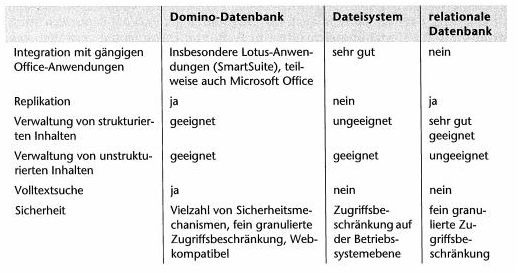
\includegraphics[scale=0.7]{pics/VorUndNachteile}}
%   \caption[Domino-Datenbanken und die Alternativen]{\label{FiG:Domino-Datenbanken und die Alternativen }
%   Domino-Datenbanken und die alternativen Möglichkeiten um Daten zu speichern im Vergleich\cite{knaepper}.}
%\end{figure}

%============================
\subsection{Datenbankarchitektur}
\label{sec:3dominoDB}

Physisch gesehen wird eine Domino-Datenbank durch eine Datei mit \textit{.nsf}-Endung abgebildet. Die Endung
\textit{.nsf} steht für Notes Storage Facility. Wie dem Namen zu entnehmen ist handelt es sich um die Möglichkeit, Notizen (Notes) aufzunehmen.
 Diese Notes, oder in anderen Worten gesagt, Dokumente oder Datensätze enthalten Felder welche mit Daten oder Informationen gefüllt sind\cite{ebel}.

\begin{figure}[H]
  \centerline{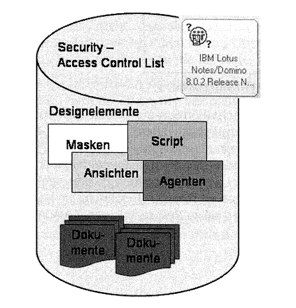
\includegraphics[scale=0.7]{pics/DB_container}}
  \caption[Elemente einer Domino-Datenbank]{\label{FiG:Elemente einer Domino-Datenbank }
  Elemente einer Domino-Datenbank\cite{ebel}.}
\end{figure}
\begin{flushleft}
Die Abbildung 3.1 zeigt den Aufbau einer Domino-Datenbank. Es ist erkennbar, wie Design-Elemente und Dokumente in einem gemeinsamen Container
abgelegt sind. 
\end{flushleft}


\vspace{1cm}
\begin{graybox}
\textbf{Information zu Dokumenten: }Dokumente bestehen aus Text, Feldern, Zahlen, Grafiken etc. Der Benutzer kann Daten eingeben, von Formeln
automatisch berechnen lassen, von anderen Anwendungen Daten importieren oder eine Verknüpfung einer anderen Anwendung erstellen. Dabei werden die
Daten dynamisch aktualisiert\cite{ebel}.
\end{graybox}

%\newline
%\begin{figure}[H]
%   \centerline{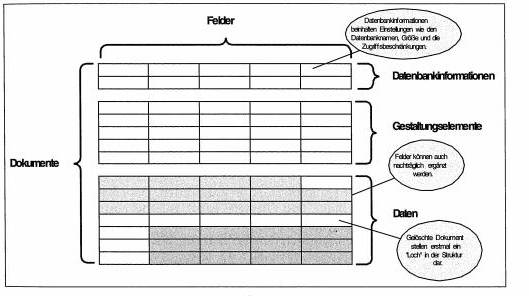
\includegraphics[scale=0.7]{pics/AufbauDominoDB}}
%   \caption[Aufbau einer Domino-Datenbank]{\label{FiG:Aufbau einer Domino-Datenbank }
%   Aufbau einer Domino-Datenbank\cite{knaepper}.}
%\end{figure}
%
%\begin{flushleft}
%  Weiters können Dokumente ihrem Typ nach, nochmals in \textbf{Datenbankinformationen}, \textbf{Gestaltungselementen} und \textbf{Daten} unterteilt werden.
%\end{flushleft}
%
%============================

\subsubsection{Datenbank-Informationen}
\label{sec:3dominoDB}

Die Datenbank-Informationen umfassen alle Eigenschaften einer Datenbank. Diese Eigenschaften sind für die gesamte Datenbank gültig.
\begin{flushleft}
Zu diesen Informationen gehören unter anderem:
\end{flushleft}
\begin{itemize}
\item Identifikation einer  Datenbank
\item Datenbanktitel
\item Name der Datenbankdatei
\item maximale Größe
\item verfügbarer Speicherplatz 
\end{itemize}
Die meisten dieser Eigenschaftseinstellungen werden beim Erstellen einer Datenbank, durch den Ersteller spezifisch, angegeben. 
Weiters besteht auch die Möglichkeit, dass die Einstellungen durch das System automatisch vorgenommen werden.

%============================
\subsubsection{Gestaltungs- oder Design-Elemente}
\label{sec:3dominoDB}

Wie in Kapitel 3.1 bereits erwähnt, besteht ein Domino-Datenbank nicht nur aus Daten sondern bietet auch eine Reihe von Gestaltungs- oder Design-Elementen.
Informationen über Design-Elemente werden ebenfalls in Dokumenten verwaltet. Dies bietet die Möglichkeit, sie zu kopieren, zu löschen oder replizieren zu
können. Die notwendigen Design-Elemente für das Template, werden in Kapitel 4.3 aufgelistet und beschrieben. 

%============================

\subsubsection{Daten}
\label{sec:3dominoDB}

Die Verwaltung der eigentlichen Daten, wird wie auch die der Design-Elemente, über Dokumente erledigt. 
Ein Dokument ist eine autonome Einheit, welche die Struktur eigenständig verwaltet. Dies hat den Vorteil, dass die Größe und die Struktur des 
Dokumentes zu jedem Zeitpunkt beliebig verändert werden kann. Dokumente besitzen die Funktion sich wie ein Behälter für Grafiken, Texte, Objekte
oder multimediale Daten zu verhalten. Diese Funktionalität wird auch als \textit{compound-document} bezeichnet und ist für relationalen Datenbanken,
nur über umständliche Wege realisierbar. Ein compound-document ist ein aus mehreren Objekten zusammengesetztes Dokument\cite{wind}. 

\vspace{0.5cm}

\begin{graybox}
\textit{In einer dokumentorientierten Umgebung wie Notes bilden compound-documents die Grundlage einer jeden Internet-/Groupware-/Workflow-Anwendung\cite{knaepper}.}
\end{graybox}



%============================



